\chapter{Proposed Framework}
As already shown, one of the main task of predictive maintenance is anomaly detection, described as a set of techniques for the identification of some anomalous warning states in which an under observation machine could be, allowing a better maintenance activities planning. In this part, the task performed is firstly formalized and then the proposed architecture is illustrated. At the end of the chapter a list of technologies used during implementation is presented.
\section{Problem definition}
In this section the performed anomalous sound detection task is formalized. The proposed framework is built to classify as normal or anomalous audio clips placed in input. The training set is composed of $K$ audio clips $\{x_1, x_2, ...,x_K\}$ in \textit{.wav} format, recorded from different versions of a machine type $M$, with a duration of $T$ seconds (for example $K$ clips from four different pumps). An ID string is used to identify the different versions of $M$. Moreover, since only few audio clips are recorded when anomalies are present, they are incorporated into a different set, used for testing purpose. For the reasons explained in previous chapters, this task cannot be solved using classification, even though it seems to be a two-class classification problem. To clarify, only one model is trained to perform anomaly detection on different versions of M, using, in training phase, normal audio clips recorded from all of them. In this way the complexity of the predictive maintenance system is reduced, because one single model can be used for different machines, avoiding repeating the training operations, in any case expensive, for each machine.\\
Before describing the proposed model in detail, let’s have a look to the implemented framework from an high level view (Figure \ref{high-level-architecture}). As it can be seen, the input consists in an audio clips recorded by microphones disposed around monitored machines, while the output is a label, \textit{normal} or \textit{anomaly}.
\begin{figure}[ht]
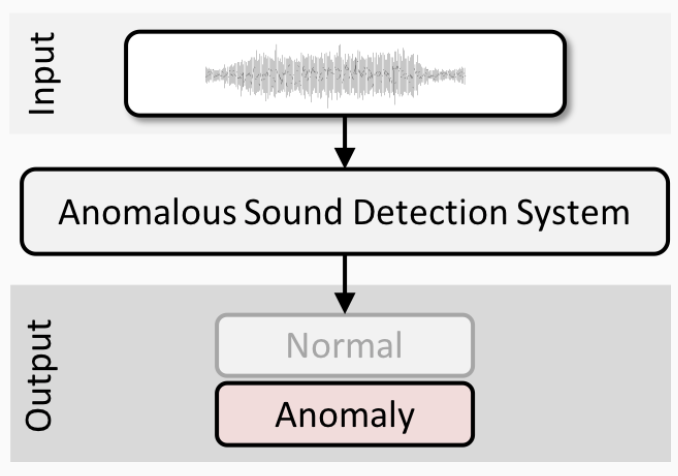
\includegraphics[scale=0.6]{TESI DI FIORE/img/high-level-architecture.png}
\centering
\caption{High level architecture \cite{DCASE}}
\label{high-level-architecture}
\end{figure}

\section{Model architecture}
The proposed ASD system operations consist of two main phases: an offline phase, responsible of autoencoder models training, and an online operation phase, to conduct a real time detection. This framework uses autoencoders to resolve the lack of anomalous data problem and uses audio features and all their advantages, as shown in Chapter 2.\\
In the next two subsections there are detailed descriptions of both phases, with a focus on each block present in the pipelines.
\subsection{Offline Training Phase}
\begin{figure}[ht]
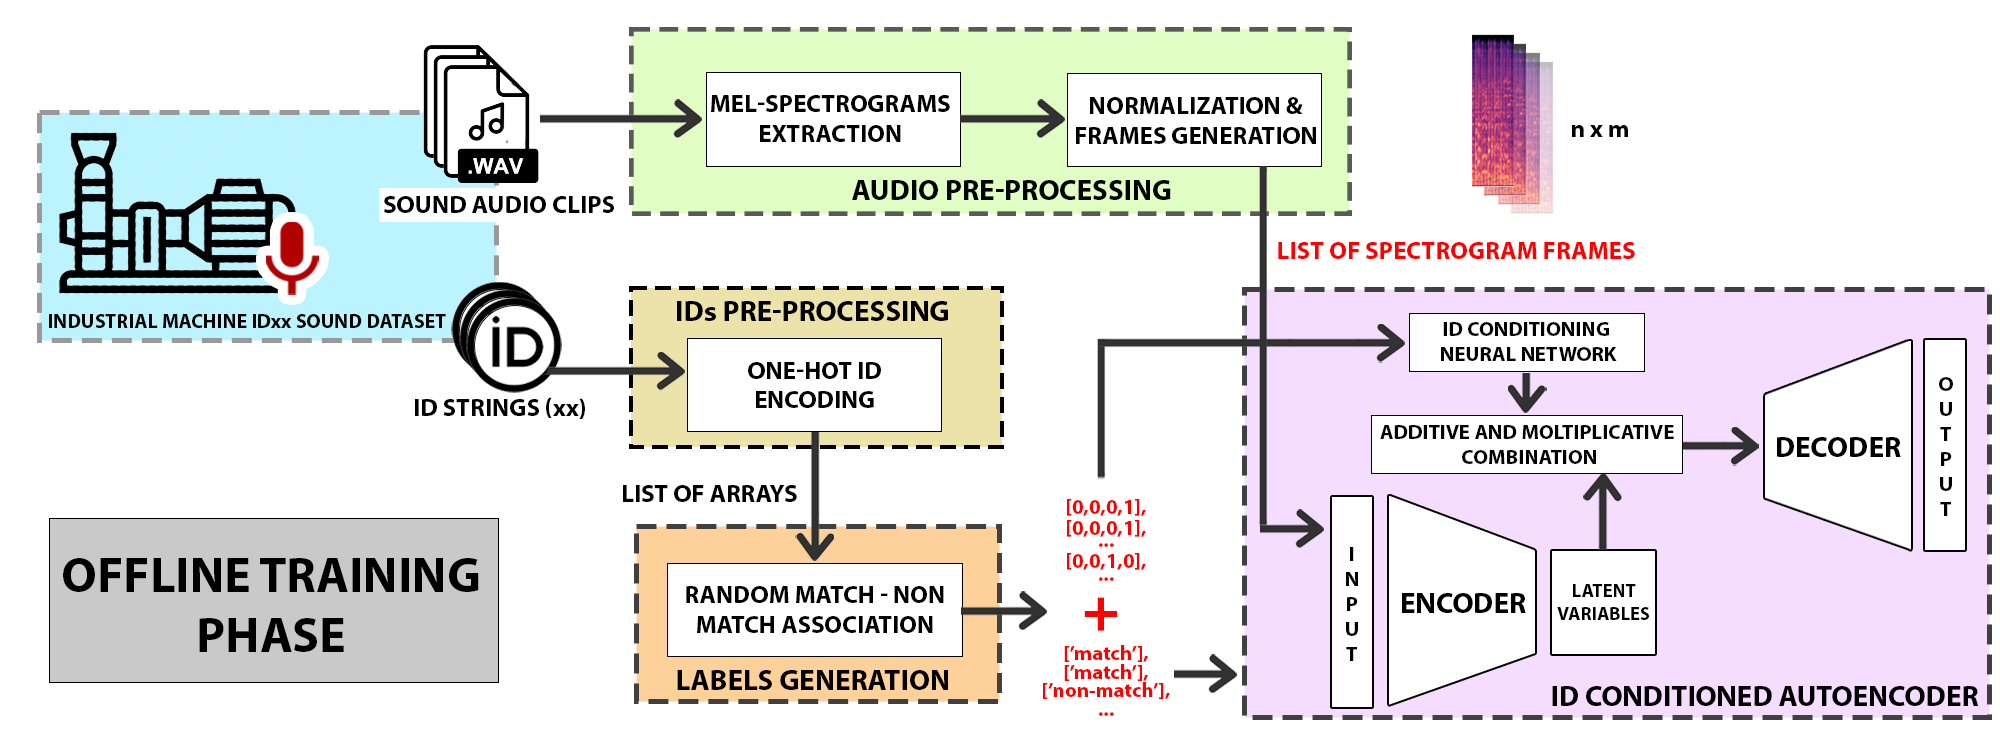
\includegraphics[scale=0.2]{TESI DI FIORE/img/offline-architecture.png}
\centering
\caption{Overview of offline training phase of the proposed ASD system.}
\label{offline-asd-system}
\end{figure}
This phase is responsible of the training of an autoencoder. The training process must be done in offline manner with the use of a pre-collected normal audio clips which belong to machines of the same type. In addition to the dataset, analyzing the Figure \ref{offline-asd-system}, other components can be noticed: the Audio Pre-Procesing block, the IDs Pre-Processing block, the Label Generation block and the ID Conditioned Autoencoder. The first three parts prepare the dataset for training process, which it is executed in the last one.
\subsubsection{Dataset Structure}
In addition to audio clips, the dataset must provide the IDs used to identify particular versions of $M$, embedding them into clips filenames (with \textit{.wav} extension) or in a separated file (obviously maintaining a one-to-one correspondence with audio files). Definitely, the data should be structured in pairs composed by audio clips plus an identifier.
\subsubsection{Offline Audio Pre-Processing}
This part of the framework is responsible of audio clips transformation, a necessary operation to make them ready for the neural network learning process, executed into the ID Conditioned Autoencoder block. There are two different components in this block:
\begin{itemize}
    \item {\textit{Mel-Spectrogram extractor} receives input audio clips and produces corresponding log-mel-scale spectrograms in output.}
    \item {\textit{Normalization and Frames generator} executes normalization on all spectrograms extracted and then it produces, from log-mel-spectrogram received in input, $n \times m$ overlapping frames with segmentation. Normalization is done on all spectrograms with the same ID. For example, in case of min-max normalization, the number of different maximum and minimum values found is equal to the number of different IDs. }
\end{itemize}
A little digression should be made about what these spectrograms are and how the first block calculate them. A signal is a variation in a certain quantity over time and for audio this quantity is air pressure, sampled by microphones with a particular rate (in the order of kHz). The Fast Fourier Transform (FFT) is an algorithm that allows the decomposition of a signal into its individual frequencies and frequency amplitudes, converting it from the time domain into the frequency domain (generating the spectrum). The Short-Time Fourier Transform (STFT) allows the representation of signals spectrum as they vary over time (generating the spectrogram). As audio signals frequency content varies over time (non-periodic signals), STFT is applied, because it is a FFT computed on overlapping windowed segments of the signal (Figure \ref{sftf}).\\
\begin{figure}[ht]
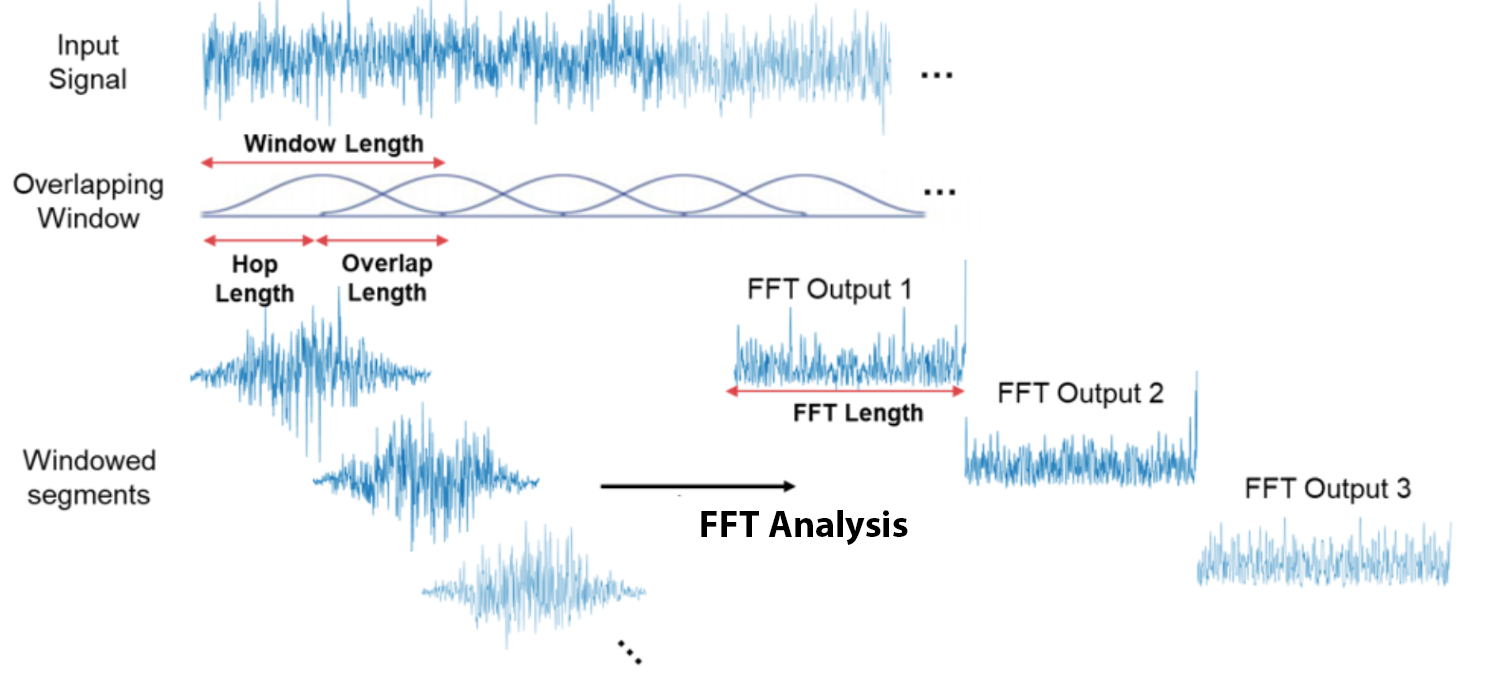
\includegraphics[scale=0.4]{TESI DI FIORE/img/STFT.png}
\centering
\caption{Overview of the STFT process.}
\label{sftf}
\end{figure}
Spectrograms usually present time on the x-axis, frequencies on the y-axis and amplitudes are indicated by colors. Log-mel-spectrograms are spectrograms in which the frequencies on y-axis are represented using the mel-scale and the amplitudes are expressed in Decibel (dB). With respect to the normal scale, the mel-scale is a scale of pitches judged by listeners to be equal in distance one from another. The most important parameters involved into this transformation process are the length of the window used for STFT ($n\_fft$), the length of the overlap between two successive windows ($hop\_length$) and the number of bins used for the transformation into the mel scale ($n$).
In the Figure \ref{features-extraction} a more detailed graphical view of what this block does is illustrated.
\begin{figure}[ht]
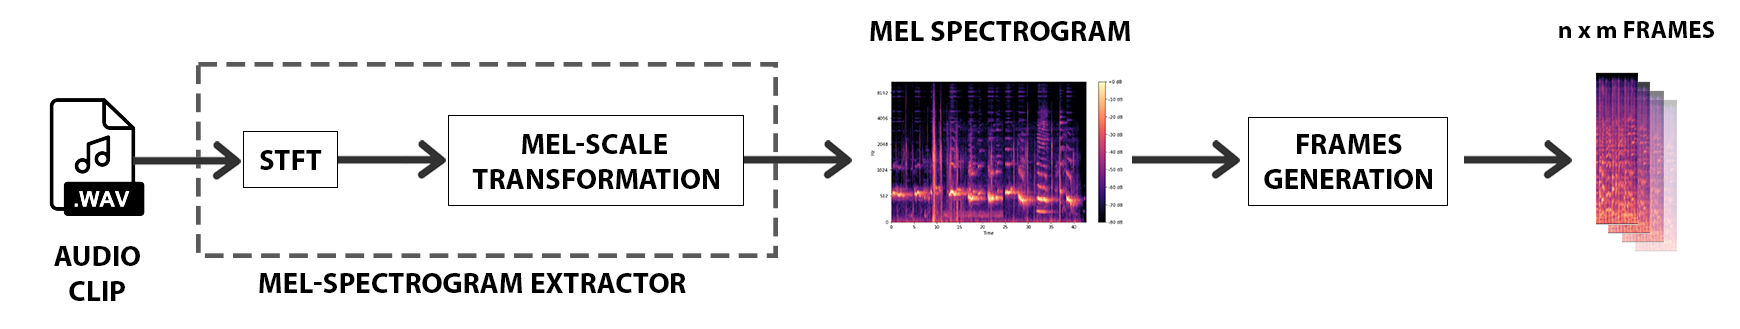
\includegraphics[scale=0.5]{TESI DI FIORE/img/FeatureExtraction.png}
\centering
\caption{Features extraction block}
\label{features-extraction}
\end{figure}
In the offline phase, $n \times m$ frames are generated from all $n \times q$ spectrograms of the training set, in order to build a new, pre-processed dataset ready for training process.
\subsubsection{IDs Pre-Processing}
This block receives in input a string, the machine ID associated to each audio clip, and converts it to a binary sequence, whose length depends by the number of different versions of $M$. This is done by the One-Hot Encoder. One-hot encoding is a technique used to convert some categorical or nominal features in order to make them compatible with training algorithm. Here ID strings are converted. Let's take an example. Supposing to have a machine $M$ and that there are four different versions of it, identified as $ID00$, $ID01$, $ID02$, $ID03$, one-hot encoder converts these strings into $[0,0,0,1]$, $[0,0,1,0]$, $[0,1,0,0]$ and $[1,0,0,0]$, respectively. The length of binary sequences is four because four is the number of versions in this case. This operation arranges the IDs to be inputs of the ID Conditioning Neural Network, better explained in the next sections. In conclusion, since each audio file spectrogram is segmented in frames, this block must ensure that those extracted from the same spectrogram are associated to the same binary sequence.
\subsubsection{ID Conditioned Autoencoder}
This part of the architecture is obviously the most important one. It receives in input three lists: the list of spectrogram frames, the list of one-hot-encoded ID arrays and the list of strings produced by Label Generator. The latter is used for the loss calculation during the training process, so that it is not a real input of the neural network (the details of what this block does are reported in the next section). In this block there are two main components: the autoencoder, composed by an encoder and a decoder, which receives the spectrogram frames in input, and the ID Conditioning Neural Network, which receives ID binary sequences. Following there is a mathematical representation of these components \cite{18IDConditionedAutoEncoder}:
\begin{itemize}
    \item {Encoder $E: \mathcal{X} \rightarrow \mathcal{Z}$ which maps the input $X$ from $\mathcal{X}$ into its encoded version $Z = E(X)$;}
    \item {Decoder $D:  \mathcal{Z} \rightarrow \mathcal{X}$ which takes the code from $\mathcal{Z}$ and outputs a reconstruction of $X$; }
    \item {Conditioning made by two functions $H_\gamma$ and $H_\beta: \mathcal{Y} \rightarrow \mathcal{Z}$, taking in input the one-hot encoded ID $l$ from $\mathcal{Y}$ in order to map it into $H_\gamma(l)$ and $H_\beta(l)$, with the same size as code from $\mathcal{Z}$.}
\end{itemize}
The encoder and the decoder can be created with different type of layers, like convolutional, LSTM or fully-connected dense layers. Between the encoder and the decoder there is a latent or encoded representation of the input $X$, or else $Z$. Differently from conventional autoencoders, in this architecture the autoencoders are conditional, because decoder input is not $Z$, but its mathematical combination with the output of conditioning functions: \[Decoder \; input: H(Z,l) = H_\gamma(l) \cdot Z + H_\beta(l).\] The conditioning functions $H_\gamma(l)$ and $ H_\beta(l)$ can be realized, for example, using dense layers and activation functions. In conclusion, the output of the entire autoencoder is $D(H(E(X),l))$. The goal of ID conditioning is to inform the model about the presence of different machines of the type $M$, for the recognition of their different normal behaviours. In general, anomalous sound of a machine $M$ with ID $x$ could be similar to normal sound of machine $M$ with ID $y$ and this could generate some false negative (FN). Moreover, normal sound of a machine $M$ with ID $w$ could be different from normal sound of a machine $M$ with ID $z$ and this could generate some false positive (FP). These two situations happen because the autoencoder is unable to separate different machine versions normal behaviour. The key concept is that the autoencoder must be trained to reconstruct normal audio spectrograms placed input only if the provided ID is correct. With this assumptions, after the training, if a normal test sample is placed in input, a low reconstruction error (in terms of mean absolute error or mean squared error) is expected, while if there is an anomalous one, an high reconstruction error is generated, even if this anomalous behavior is similar to a normal behaviour of another machine, thanks to the presence of the ID. The similarity problem is so resolved by the presence of the ID. 
\subsubsection{Label Generation}
At this point a question arises: are the only ID conditioning operations enough for this task? The answer is no because is necessary to edit the training process to help the autoencoder in the recognition of the relationship between IDs and audio clips. For this reason there is the Label Generation block. This block, for each frame, randomly changes with a probability $1-\alpha$ the correct associated ID binary sequence and it adds the string \textit{match} or \textit{not-match} on the basis of decisions. For example if there are 100 audio clips and $\alpha$ is 0.75, 75 audio clips will be associated to the correct ID sequence, the remaining 25 will be associated to a random one, from those available (so that frames belonging to the same spectrogram have the same ID binary sequence and the same string). Moreover, in order obtain what it has been just described, a new loss must be tuned and used in training steps because the classical difference between the encoder input and the decoder output is not enough. In fact, to allow a good reconstruction of the input only when the associated ID is correct, during the training, if the label is \textit{match} the loss function must be calculated in classical way as $||D(H(E(X),l)) - X||$,
while if the label is \textit{not-match} the loss function must be calculated using an arbitrary vector C: $||D(H(E(X),l)) - C||$.
In conclusion, when the input spectrogram frames are associated to wrong IDs, the autoencoder will generate an high reconstruction error.
\subsection{Online Operation Phase}
\begin{figure}[ht]
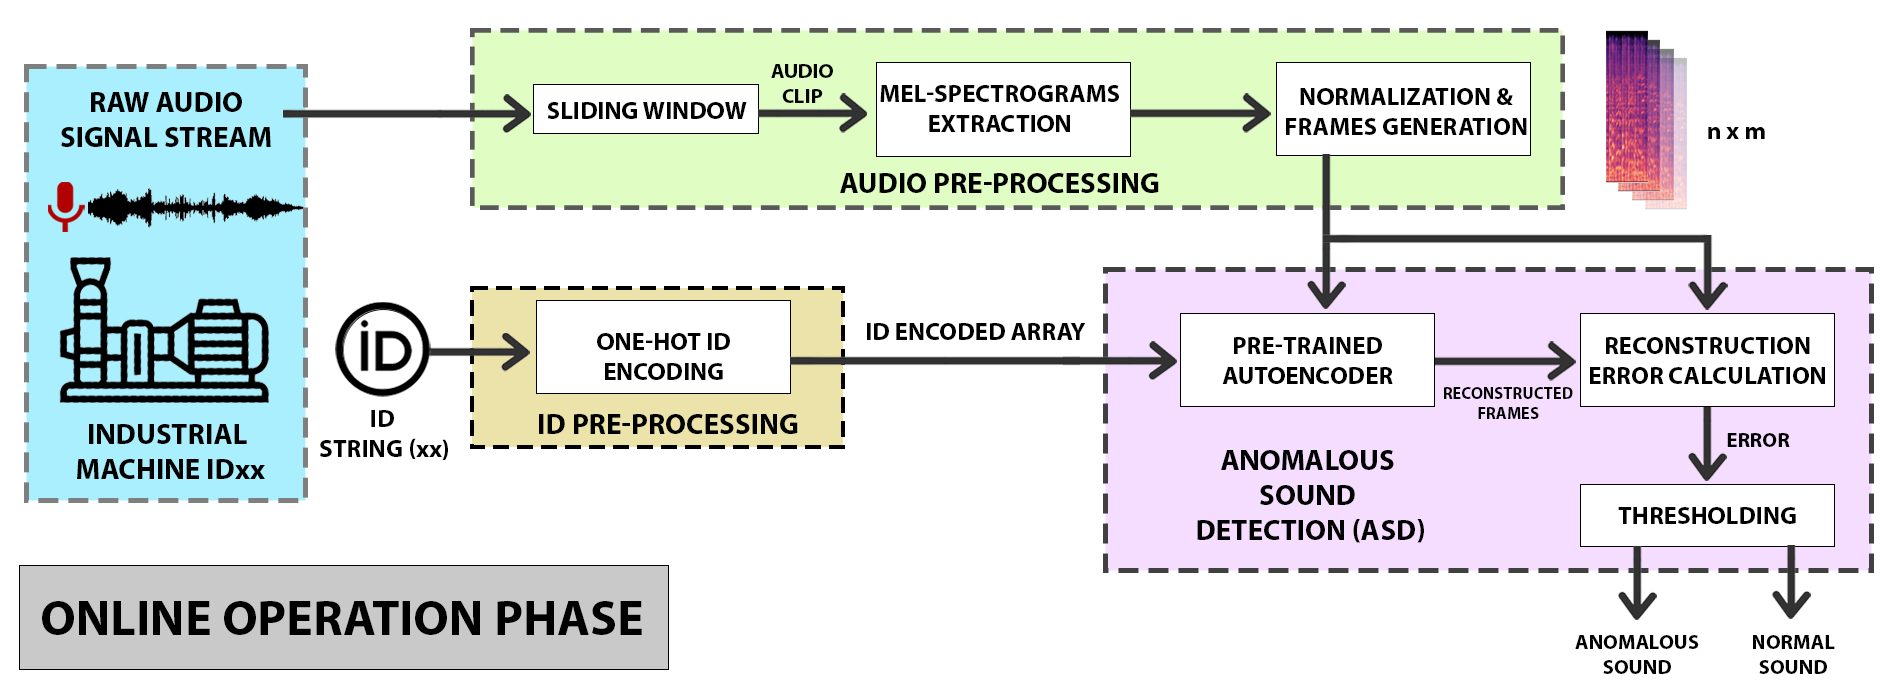
\includegraphics[scale=0.9]{TESI DI FIORE/img/online-architecture.png}
\centering
\caption{Overview of online operating phase of the proposed ASD system, trained on machine with ID equal to xx}
\label{online-asd-system}
\end{figure}
The architecture used for online operation phase is very similar to the part just described, except for few components. This part of the architecture is meant for an effective and an operative use on field, since the left part of the Figure \ref{online-asd-system} shows that there is not a dataset but a real time raw audio stream from microphones disposed around the machine $M$. As other elements have been already explored in previous sections, following  there is only a description of the new ones and those that are different: Online Audio Pre-Processing block and the Anomalous Sound Detection block. 
\subsubsection{Online Audio Pre-Processing}
It is very similar to the one presented before, with exception of the sliding window component. Because of real-time anomaly detection, there is a continuous audio stream, but the autoencoder model is implemented and trained to work with $T$ seconds audio clips. For this reason, the sliding window component takes in input the stream and samples the last $T$ seconds from it, every $h$ seconds. Next, previously obtained audio clips pass into mel-spectrogram extractor block and into the frame generator, already presented. 
\subsubsection{Anomalous Sound Detection}
This is the final block of the online part of the framework and the one that is responsible of the sound labeling as normal or anomalous. In this part three components are highlighted: the pre-trained autoencoder, the reconstruction error calculator and a threshold. The pre-trained autoencoder is the result of the operations made by the offline part of the architecture. The reconstruction error calculator takes in input the output of the autoencoder and its input in order to evaluate the difference between them, in terms of MAE or MSE. This operation is made for each frame of the spectrogram associated to the audio clip (sampled from the stream) and then an average of recostruction errors is calculated for the comparison with the threshold. In fact, the threshold is used to establish if the average reconstruction error is high enough to classify clips as anomalous. The threshold could be chosen using reconstruction errors of training samples or using different approaches based on ROC curves, like the one presented at the end of Chapter 4.
\section{Hyperparameters}
In order to give a better idea related to the hyperparameters of the proposed model, following there is a summary of the most important ones:
\begin{itemize}
    \item {\textit{C}: the constant vector that must be reconstructed by the autoencoder when the provided ID is wrong;}
    \item {$\alpha$: the percentage of correct frame-ID couples in training set;}
    \item {\textit{NUM\_CONDITIONING\_LAYERS}: number of layers of the conditioning neural network;}
    \item {\textit{NUM\_CONDITIONING\_NEURONS}: number of neurons used in the the conditioning layers of the neural network and also the dimension of the encoded input generated by the encoder.}
\end{itemize}
Clearly, because of the architecture is compatible with different implementations of autoencoder layers, other hyperparameters that arise from them should be taken in consideration. Moreover, there are other hyperparameters, such as learning rate, batch size and number of epochs, which are not dependent on the proposed architecture but affect the training phase of the model.
\section{Implementation technologies}
In this section, some implementation details about the proposed model are given. The model was implemented in Python 3. Used technologies and libraries are:
\begin{itemize}
    \item {Google Colab\footnote{http://colab.research.google.com}: Colab notebooks are Jupyter notebooks that run in the cloud and are highly integrated with Google Drive, making them easy to set up, access, and share;}
    \item {Tensorflow\footnote{https://www.tensorflow.org}: it is an end-to-end open source platform for Machine Learning;}
    \item {Keras\footnote{https://keras.io}: it is an open source Deep Learning API written in Python3;}
    \item {NumPy\footnote{https://numpy.org}, used to work in an efficient way with arrays;}
    \item {SciKit-Learn\footnote{https://scikit-learn.org/stable/}, a machine learning library, containing simple and efficient tools for predictive data analysis;}
    \item {Librosa\footnote{https://librosa.org}, a Python library for audio and music processing.}
\end{itemize}

